\chapter{Planificación, metodología y presupuesto del proyecto}

Este capítulo tiene como objetivo describir el enfoque metodológico adoptado para el desarrollo del proyecto, así como la planificación temporal y los recursos necesarios para su ejecución. La correcta organización del trabajo es fundamental para garantizar una implementación coherente, eficiente y ajustada a los objetivos establecidos.

En primer lugar, se expone la metodología empleada para estructurar y gestionar el proyecto, en este caso basada en principios de desarrollo ágil, concretamente mediante la utilización del marco SCRUM. Esta elección permite una adaptación progresiva a los retos que puedan surgir, promoviendo la flexibilidad y la mejora continua a lo largo del proceso.

A continuación, se presenta la planificación detallada del proyecto, dividida en varias iteraciones que abarcan desde la fase de análisis inicial hasta la validación de los resultados obtenidos. Se especifican las tareas previstas en cada etapa, su duración estimada y su prioridad, lo que facilita el seguimiento del avance del proyecto.

Finalmente, se ofrece una estimación del presupuesto necesario, teniendo en cuenta tanto los recursos materiales como los costos asociados al tiempo de dedicación. Aunque se trata de un trabajo académico, este ejercicio resulta útil para valorar la viabilidad del proyecto en un contexto profesional real.

\section{Metodología utilizada}
Para la organización y desarrollo de este TFG se ha optado por seguir el marco de trabajo SCRUM. Esta elección permite estructurar el proyecto en ciclos iterativos e incrementales, favoreciendo la adaptabilidad, el control del progreso y la mejora continua.

El proyecto se ha dividido en tres iteraciones principales, cada una con una duración determinada y unos objetivos específicos. 

Esta planificación permite mantener una visión clara del desarrollo del trabajo, asegurando que se cumplen los plazos establecidos y que se cubren progresivamente todos los aspectos necesarios del proyecto, desde la recolección y análisis de datos hasta el diseño y validación del modelo propuesto.

En total, se han definido 17 historias de usuario para el proyecto. Cada una de ellas cuenta con una estimación del esfuerzo necesario, basada en la escala de Fibonacci. Además, se les ha asignado un nivel de prioridad, que puede ser: muy alta, alta, media o baja. Las historias están ordenadas según el cronograma previsto de desarrollo, aunque este orden puede modificarse en función de las necesidades del proyecto.

\begin{table}[h]
    \centering
    \begin{tabular}{|>{\centering\arraybackslash}p{1.5cm}|>{\centering\arraybackslash}p{6cm}|>{\centering\arraybackslash}p{2cm}|>{\centering\arraybackslash}p{1.8cm}|}
        \hline
        \textbf{ID} & \textbf{Historia de Usuario} & \textbf{Prioridad} & \textbf{Estimación} \\ \hline
        HU.01 & Reunión inicial con tutores & Muy alta & 2 \\ \hline
        HU.02 & Revisión de la literatura & Alta & 13\\ \hline
        HU.03 & Redacción del estado del arte& Alta & 8\\ \hline
        HU.04 & Definición de las estadísticas a almacenar & Alta & 3 \\ \hline
        HU.05 & Diseño de la base de datos & Alta & 5\\ \hline
        HU.06 & Implementación de programa para recolectar datos & Alta & 8\\ \hline
        HU.07 & Diseño de algoritmo para definir ganador por pesos& Alta & 8 \\ \hline
        HU.08 & Implementación algoritmo para definir ganador por pesos& Alta & 5\\ \hline
        HU.09 & Implemetación programa básico sin pesos & Media & 2 \\ \hline
        HU.10 & Análisis de las variables del agoritmo genético & Media & 5 \\ \hline
        HU.11 & Implementación del algoritmo genético por pesos & Alta & 5 \\ \hline
        HU.12 & Implementación del algoritmo genético por pesos y $\delta$ & Alta & 5 \\ \hline
        HU.13 & Análisis de los datos recogidas por los algoritmos& Alta & 8\\ \hline
        HU.14 & Diseño algoritmo para obtención de datos individuales del partido & Baja & 3 \\ \hline
        HU.15 & Implemetación del algoritmo para obtención de datos individuales del partido& Baja & 5 \\ \hline
        HU.16 & Análisis de los datos de cada jugador individual& Baja & 5 \\ \hline
        HU.17 & Redacción de la memoria & Alta & 8 \\ \hline
    \end{tabular}
    \caption{Listado inicial de tareas}
    \label{tab:placeholder_label}
\end{table}

La manera en la que se han dividido las historias en las distintas iteraciones ha sido la siguiente:
\begin{itemize}
    \item Iteración 1: HU.01, HU.02, HU.03, HU.04, HU.05 (31 puntos de historia)
    \item Iteración 2: HU.06, HU.07, HU.08, HU.09, HU.10, HU.11 (33 puntos de historia)
    \item Iteración 3: HU.12, HU.13, HU.14, HU.15, HU.16, HU.17 (34 puntos de historia)
    
\end{itemize}

Las historias se han dividido para intentar que haya un número similar de puntos de historia en cada iteración. 

La primera iteración, que es la que menos tiene, sirve también para inicializarme en el proyecto con la reunión inicial con tutores, la revisión del estado del  arte y su redacción, la decisión de las estadísticas a almacenar y el diseño que tendría la base de datos.

La segunda iteración se basa principalmente en la implementación de los algoritmos del programa, y la tercera iteración en la implementación del último algoritmo, de su análisis, lo relativo al rendimiento individual de cada jugador y la redacción de la memoria.

Se han intentado dividir las historias para que cada iteración siga una única temática y, al mismo tiempo, seguir un orden en la realización del proyecto.

\section{Temporización}
Para la temporización se ha decidido asignarle a cada iteración un tiempo de 4 semanas, empezando el día 1 de marzo y acabando el 31 de mayo, es decir, a cada iteración le pertenece un mes aproximadamente. Dentro de cada iteración se ha dividido el tiempo conveniente para cada historia, haciendo primero aquellas que son necesarias para continuar. El diagrama de Gantt de todo el proyecto se puede ver en la siguiente página.

\begin{figure}[p]
    \centering
    \begin{sideways}
        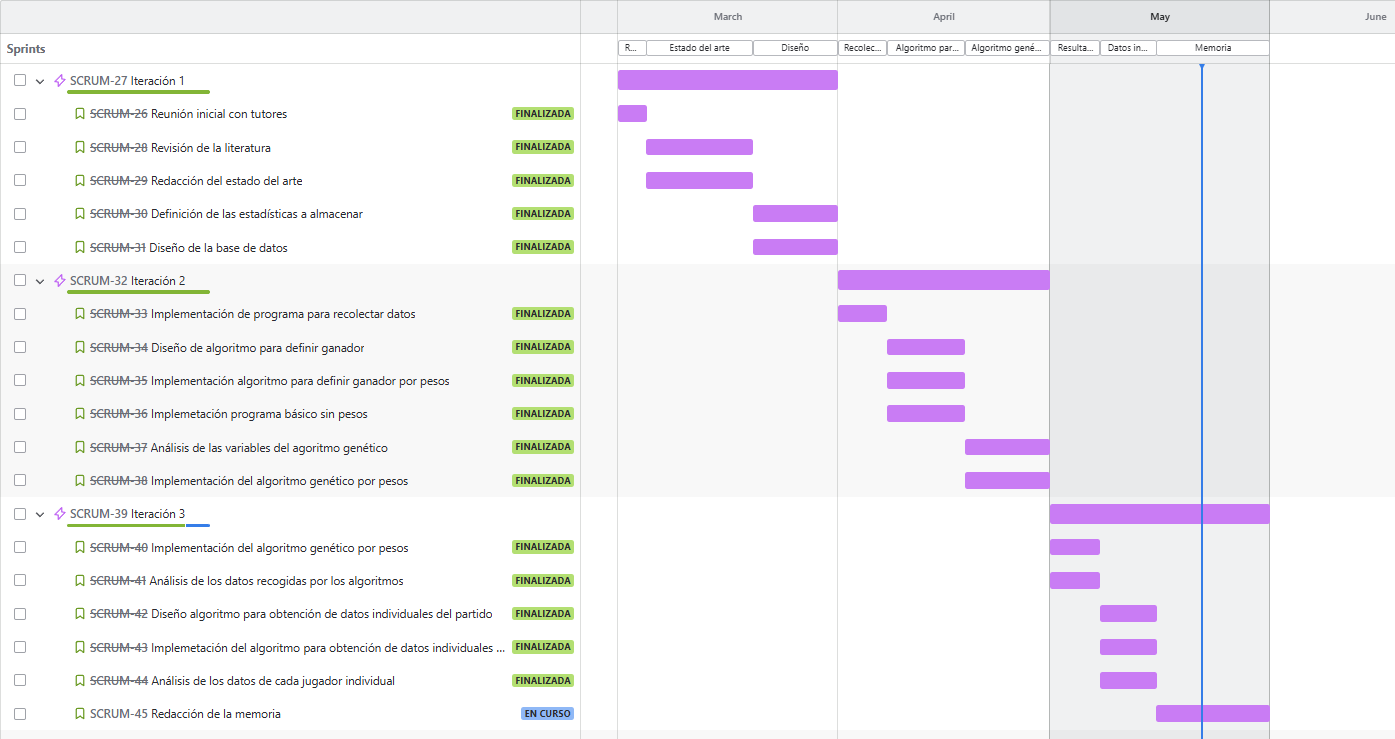
\includegraphics[width=\textheight, height=\textwidth, keepaspectratio]{plantilla-TFG-ETSIIT/doc/imagenes/Diagrama-Gantt.png}
    \end{sideways}
    \caption{Diagrama de Gantt del proyecto}
    \label{fig:imagen-ajustada}
\end{figure}

\section{Presupuesto}
\subsection*{Coste de personal}
Para este proyecto se necesita la contratación de un informático junior. Según la página web talent \cite{sueldo-junior}, el sueldo de un programador junior en España es de 13,46 €/hora, a lo que hay que sumarle un aproximado 25\% por seguro médico, IRPF y demás impuestos, lo que lo deja en 16,83 €/hora. Durante este proyecto se ha trabajado durante 300 horas aproximadamente. También se necesita a un ingeniero en sistemas para mantener el servidor, según \cite{sueldo-sistemas} su sueldo medio es de 24,20 €/hora más un 25\% aproximado otra vez por impuestos, y ha trabajado 1 hora al día para verificar que todo estaba bien durante los 2 últimos meses del proyecto. También se va a prever 1 año más para dar soporte al proyecto y que pueda mantenerse.

\begin{table}[h!]
\centering
\begin{tabular}{|c|c|c|c|}
\hline
\textbf{Descripción} & \textbf{Horas} & \textbf{€/hora} & \textbf{Coste(€)} \\
\hline
Programador junior & 300 & 16,83 & 5.047,5 \\
\hline
Ingeniero en sistemas & 425 & 30,25 & 12.856,25 \\
\hline
Total &  &  & 17.903,75 \\
\hline
\end{tabular}
\caption{Coste de personal}
\label{tab:ejemplo}
\end{table}

\subsection*{Coste de material}
En cuanto a hardware, se ha hecho de un portátil Lenovo Ideapad Gaming 3 cuyo coste de compra fue de 900 €. Hace 4 años que se compró, pero solo se va a usar durante un año, debido al mantenimiento del servidor. Simulando que se vaya a lanzar este proyecto de manera profesional, también se necesita el uso de un servidor con capacidad para albergar gran cantidad de datos. Se ha utilizado un servidor físico (HPE ProLiant MicroServer Gen10+) como plataforma para alojar la base de datos MongoDB, con un coste estimado de 775.98 €. Esto permite replicar un entorno profesional con servicios persistentes y seguros de gestión de datos.

En cuanto a software, se hace uso de MongoDB, Visual Studio, GitHub y Ubuntu; todos son gratuitos.

\begin{table}[h!]
\centering
\begin{tabular}{|c|c|c|c|c|}
\hline
\textbf{Descripción} & \textbf{Coste(€)} & \textbf{Años} & \textbf{Años usado} & \textbf{Coste(€)} \\
\hline
Portátil & 900 & 5 & 1 & 180 \\
\hline
Servidor & 775,98 & 1 & 1 & 775,98 \\
\hline
MongoDB & 0 & 1 & 1 & 0 \\
\hline
Visual Studio & 0 & 1 & 1 & 0 \\
\hline
GitHub & 0 & 1 & 1 & 0 \\
\hline
Ubuntu & 0 & 1 & 1 & 0 \\
\hline
Total &  & & & 955,98 \\
\hline
\end{tabular}
\caption{Coste de material}
\label{tab:ejemplo}
\end{table}

\subsection*{Costes indirectos}
Para los costes indirectos se estima un 10\% del gasto total del proyecto.
\begin{table}[h!]
\centering
\begin{tabular}{|c|c|c|c|}
\hline
\textbf{Descripción} & \textbf{Total} & \textbf{\%} & \textbf{Coste(€)} \\
\hline
Costes indirectos & 18.859,73 & 10 & 1.527,89 \\
\hline
Total &  &  & 20.745,70 \\
\hline
\end{tabular}
\caption{Costes indirectos}
\label{tab:ejemplo}
\end{table}

El coste total del proyecto sería de 20.745,70 €.